\documentclass[9pt]{beamer}
%\documentclass[handout]{beamer}

\usetheme{default}
\usecolortheme{dove}
\usefonttheme{professionalfonts}

\usepackage[utf8]{inputenc}
\usepackage{csquotes}
\usepackage[ngerman]{babel}
\usepackage[backend=biber,style=numeric,sorting=nyvt]{biblatex}
\usepackage{tikz}
\usetikzlibrary{arrows,shapes,shapes.geometric,positioning}
\usepackage[export]{adjustbox}
\usepackage{pifont}
\usepackage{epigraph}
\usepackage{graphbox}
\usepackage{array}

\definecolor{FrameColor}{HTML}{0880be}
\definecolor{HighlightColor}{HTML}{08496d}
\definecolor{WarnColor}{HTML}{f07070}

%%%% BEGIN Custom Styling %%%%

\setbeamersize{text margin left=5mm,text margin right=5mm}

%\useinnertheme{rectangles}
%\useoutertheme{infolines}

\usepackage{fontspec}
\setsansfont{DeJaVuSans}

\setbeamercolor{itemize item}{fg=black}
\setbeamercolor{itemize subitem}{fg=black}
\setbeamercolor{itemize subsubitem}{fg=black}
\setbeamertemplate{itemize item}{\scriptsize\raise1.25pt\hbox{\textbullet}}
\setbeamertemplate{itemize subitem}{\tiny\raise1.5pt\hbox{\textbullet}}
\setbeamertemplate{itemize subsubitem}{\tiny\raise1.5pt\hbox{\textbullet}}
\setbeamertemplate{enumerate item}{\insertenumlabel.}
\setbeamertemplate{enumerate subitem}{\insertenumlabel.\insertsubenumlabel}
\setbeamertemplate{enumerate subsubitem}{%
  \insertenumlabel.\insertsubenumlabel.\insertsubsubenumlabel}
\setbeamertemplate{enumerate mini template}{\insertenumlabel}

% footer
\beamertemplatenavigationsymbolsempty

\setbeamertemplate{frametitle}{\textbf{\insertframetitle}\hfill}

\setbeamertemplate{footline}{%
  \begin{center}
    \color{FrameColor}
    \rule{0.93\textwidth}{0.05cm}
  \end{center}
  \vspace{-0.2cm}
  \hspace{0.5cm}%
  %\includegraphics[align=l, height=0.4cm]{../../images/project-logo.png}%
  \color{FrameColor}%
  \textbf{\fontsize{7}{7}\selectfont\raisebox{0.15cm}{GPN22 | 30.05.2024}}%
  \hfill%
  \usebeamercolor[fg]{page number in head/foot}%
  \usebeamerfont{page number in head/foot}%
  \selectfont\raisebox{0.15cm}{\insertframenumber\,/\,\inserttotalframenumber\kern1em}%
  \hfill%
  \color{FrameColor}%
  \textbf{\fontsize{8}{8}\selectfont\raisebox{0.15cm}{soundpaint.org}}%
  \hspace{0.45cm}{\ }
}

\newcommand{\clr}{HighlightColor}%

\setmainfont[
  Path = /usr/share/fonts/truetype/freefont/,
  Extension = .ttf,
  Ligatures = TeX
]{FreeSans}

%%%% END Custom Styling %%%%

\newcommand{\cmark}{\ding{51}}%
\newcommand{\qmark}{\ding{51} / \ding{55}}%
\newcommand{\xmark}{\ding{55}}%
\newcommand{\imply}{$\Rightarrow$}

% Add command "\danger" for a warning symbol.  Depending on your LaTeX
% distribution, you may need to run "sudo apt-get install
% texlive-fonts-extra" to make the following lines work.
\newcommand*{\TakeFourierOrnament}[1]{{%
\fontencoding{U}\fontfamily{futs}\selectfont\char#1}}
\newcommand*{\danger}{\TakeFourierOrnament{66}}

\title[Pico Simple Stupid Synth]{Pico Simple Stupid Synth}
\subtitle{Projektkurzvorstellung mit anschließender Diskussion}
\author{Jürgen Reuter}
\institute[\tt{soundpaint.org}]{\tt{soundpaint.org}}
\date[GPN22]{GPN 22\\30.~Mai 2024}

\AtBeginSection[] {
  \begin{frame}[t]{Überblick}
    \tableofcontents[currentsection]
  \end{frame}
}

\addbibresource{../../bib/gpn22.bib}

%\listfiles % DEBUG: show package versions in log

\begin{document}

\tikzstyle{every picture}+=[remember picture]
\everymath{\displaystyle}

\addtocounter{framenumber}{-1}

\begin{frame}[plain]
  \maketitle
\end{frame}

%\begin{frame}[t]{Überblick}
%  \tableofcontents
%\end{frame}

%\section{Ziele}

\begin{frame}[t]{Ziele}
  \begin{itemize}
  \item<2-> \color<2>{\clr} Pico als MIDI USB Device
  \item<3-> \color<3>{\clr} Proof-of-Concept MIDI Synth
  \item<4-> \color<4>{\clr} schnelle, einfache Synthese
  \item<5-> \color<5>{\clr} mindestens ca. 32-stimmig
  \item<6-> \color<6>{\clr} Audio-Ausgang via I²S oder analog
  \end{itemize}
\end{frame}

%\section{Architektur}

\begin{frame}[fragile,t]{USB-Schnittstelle}
  \begin{itemize}
  \item<2-> \color<2>{\clr} USB-Implementierung über
    \texttt{tinyusb}-Bibliothek (im Pico SDK enthalten)
  \item<3-> \color<3>{\clr} Gerätedefinition in Datei
    \texttt{usb\_descriptors.c}\\(TODO: Update auf \texttt{tinyusb}
    Version 0.15.x)
  \item<4-> \color<4>{\clr} Spannung über USB-Kabel beim Verbinden mit
    USB Host
  \item<5-> \color<5>{\clr} {\imply} Pico bootet, meldet sich beim
    Host als {\em Pico Simple Stupid Synth}
  \item<6-> \color<6>{\clr} {\imply} unmittelbar danach sichtbar im
    Betriebssystem
  \item<7-> \color<7>{\clr} Dispatch eingehender MIDI-Events in MIDI
    State Machine über \texttt{rx\_task()}
  \item<8-> \color<8>{\clr} Implementierung {\em Active Sensing} in
    \texttt{tx\_task()}
  \end{itemize}
  \begin{block}{Linux Shell}<6->
    \color<6>{\clr}\small
\begin{verbatim}
$ aplaymidi -l
Port    Client name                      Port name
14:0    Midi Through                     Midi Through Port-0
20:0    Pico Simple Stupid Synth         Pico Simple Stupid Synth MIDI 1
\end{verbatim}
  \end{block}
\end{frame}

\begin{frame}[t,fragile]{Hauptschleife}
  \begin{itemize}
  \item<2-> \color<2>{\clr} periodisch drei Aktivitäten
    \begin{itemize}
    \item<3-> \color<3>{\clr} ausgehende USB-Daten senden, soweit vorhanden
    \item<4-> \color<4>{\clr} eingehende USB-Daten verarbeiten, soweit vorhanden
    \item<5-> \color<5>{\clr} {\imply} MIDI State Machine aktualisiert
    \item<6-> \color<6>{\clr} nächsten Audiodatenpuffer befüllen, sofern Zeit gekommen
    \end{itemize}
  \end{itemize}
  \begin{block}{Hauptschleife (auf 1. CPU Core)}<2->
    \color<2>{\clr}\normalsize
\begin{verbatim}
void
Simple_stupid_synth::main_loop()
{
  for (;;) {
    _midi_state_machine->tx_task();
    _midi_state_machine->rx_task();
    synth_task();
  }
}
\end{verbatim}
  \end{block}
  \tikz[remember picture, overlay] {
    \node at (current page.south west) {
      {\color<3>{red}
        \begin{tikzpicture}[remember picture, overlay]
          \draw<3>[draw=red,thick] (1.1cm, 4.10cm) rectangle ++(5.3cm, 0.35cm);
        \end{tikzpicture}
      }
    };
    \node at (current page.south west) {
      {\color<4>{red}
        \begin{tikzpicture}[remember picture, overlay]
          \draw<4>[draw=red,thick] (1.1cm, 3.70cm) rectangle ++(5.3cm, 0.35cm);
        \end{tikzpicture}
      }
    };
    \node at (current page.south west) {
      {\color<6>{red}
        \begin{tikzpicture}[remember picture, overlay]
          \draw<6>[draw=red,thick] (1.1cm, 3.35cm) rectangle ++(2.3cm, 0.35cm);
        \end{tikzpicture}
      }
    }
  }
\end{frame}

\begin{frame}[t]{MIDI State Machine}
  \begin{itemize}
  \item<2-> \color<2>{\clr} wertet eingehende MIDI-Events aus
  \item<3-> \color<3>{\clr} sendet ggf. MIDI-Events zurück
  \item<4-> \color<4>{\clr} bislang nur {\em Note On} und {\em Note
    Off} unterstützt
  \item<5-> \color<5>{\clr} aktuell alles auf einen einzigen Kanal
    gemerged
  \item<6-> \color<6>{\clr} {\imply} ggf. Noten zu kurz, wenn {\em
    Note Off} aus einst anderem Kanal zuschlägt (FIXME)
  \item<7-> \color<7>{\clr} Ergebnis dennoch beachtlich ({\imply}
    Demo)
  \item<8-> \color<8>{\clr} {\em Note On} und {\em Note Off} triggern
    LED
  \item<9-> \color<9>{\clr} {\imply} primitive Aktivitätsanzeige
  \end{itemize}
\end{frame}

\begin{frame}[t]{Warum nur Rechteckschwingungen?}
  \begin{itemize}
  \item<2-> \color<2>{\clr} einfachste denkbare ``digitale''
    Schwingung
  \item<3-> \color<3>{\clr} nur zwei Sample-Werte (abh.\ von
    Lautstärke)
  \item<4-> \color<4>{\clr} Tonhöhe entspricht Frequenz
    (logarithmisch)
    \begin{itemize}
    \item<5-> \color<5>{\clr} Periodendauer $T$
    \item<6-> \color<6>{\clr} Frequenz $f$
    \item<7-> \color<7>{\clr} $f = \frac{1}{T}$
    \end{itemize}
  \item<8-> \color<8>{\clr} Lautstärke entspricht Amplitude
    (logarithmisch)
  \item<9-> \color<9>{\clr} {\imply} bei Flanke das Amplituden-Delta
    zu Ausgangsumme addieren, weiter nichts zu tun
  \end{itemize}
\end{frame}

\begin{frame}[t,fragile]{Exkurs: Linien-Rasterung (ad hoc)}
  \begin{itemize}
  \item<2-> \color<2>{\clr} Linie $y=ax+b$ für $x_0\leq x \leq x_1$
    auf Rasterbildschirm
  \item<3-> \color<3>{\clr} o.B.d.A. Annahme:
    \begin{itemize}
    \item<4-> \color<4>{\clr} Steigung $0 \leq a \leq 1$
    \item<5-> \color<5>{\clr} andernfalls: Achsen spiegeln
    \end{itemize}
  \item<6-> \color<6>{\clr} naiv:
\begin{verbatim}
for (int x = x0; x <= x1; x++) {
  const double y = a * x + b;
  draw_pixel(x, round(y));
}
\end{verbatim}
  \item<7-> \color<7>{\clr} Multiplikation, Fließkommaarithmetik
  \item<8-> \color<8>{\clr} {\imply} laaaangsamer Code\\(bei
    Prozessoren ohne Fließkommaarithmetik)!
  \end{itemize}
\end{frame}

\begin{frame}[t,fragile]{Exkurs: Linien-Rasterung (Bresenham)}
  \begin{itemize}
  \item<2-> \color<2>{\clr} initial:
  \begin{itemize}
  \item<3-> \color<3>{\clr} Konstante $y_0 = \textrm{round}(ax_0+b)$
  \item<3-> \color<3>{\clr} Konstante $y_1 = \textrm{round}(ax_1+b)$
  \item<4-> \color<4>{\clr} Konstante $dx = x_1 - x_0$
  \item<4-> \color<4>{\clr} Konstante $dy = y_1 - y_0$
  \item<5-> \color<5>{\clr} Variable $err = dx / 2$
  \item<6-> \color<6>{\clr} Variable $y = y_0$
  \end{itemize}
  \item<7-> \color<7>{\clr} Schleife:
\begin{verbatim}
draw_pixel(x0, y0);
for (int x = x0 + 1; x <= x1; x++) {
  err += dy;
  if (err >= dx) {
    y += 1;
    err -= dx;
  }
  draw_pixel(x, y);
}
\end{verbatim}
  \item<8-> \color<8>{\clr} {\imply} in der Schleife: keine
    Fließkommaarithmetik, keine Multiplikation
  \item<9-> \color<9>{\clr} {\imply} schnell :-)
  \item<10-> \color<10>{\clr} mehr Details z.B. im Wikipedia-Artikel
    ``Bresenham-Algorithmus''
  \end{itemize}
\end{frame}

\begin{frame}[t,fragile]{Rendering: Implementierung}
  \begin{itemize}
  \item<2-> \color<2>{\clr} pro Tonhöhe (Oszillator) ein Datensatz
  \item<3-> \color<3>{\clr} \texttt{count\_wrap}
    \begin{itemize}
    \item<4-> \color<4>{\clr} entspricht dem $dx$ beim
      Bresenham-Algorithmus
    \item<5-> \color<5>{\clr} initialisiert auf \texttt{round(0.5 *
      count\_inc * sample\_freq / pitch\_freq)}
    \item<6-> \color<6>{\clr} Faktor \texttt{0.5} weil 2 Flanken pro
      Periode
    \item<7-> \color<7>{\clr} \texttt{count\_inc} Zeitfortschritt zum
      jeweils nächsten Sample
    \end{itemize}
  \item<8-> \color<8>{\clr} \texttt{count} entspricht dem Fehler
    \texttt{err} bei Bresenham
  \item<9-> \color<9>{\clr} \texttt{amplitude} entspricht der
    aktuellen Auslenkung
  \end{itemize}
  \small
\begin{verbatim}
  typedef struct {
    uint32_t count_wrap;
    uint32_t count;
    uint8_t velocity;
    int16_t amplitude;
  } pitch_status_t;
\end{verbatim}
  \tikz[remember picture, overlay] {
    \node at (current page.south west) {
      {\color<3-5>{red}
        \begin{tikzpicture}[remember picture, overlay]
          \draw<3-5>[draw=red,thick] (1.1cm, 4.70cm) rectangle ++(3.1cm, 0.3cm);
        \end{tikzpicture}
      }
    };
    \node at (current page.south west) {
      {\color<8>{red}
        \begin{tikzpicture}[remember picture, overlay]
          \draw<8>[draw=red,thick] (1.1cm, 4.40cm) rectangle ++(2.4cm, 0.3cm);
        \end{tikzpicture}
      }
    };
    \node at (current page.south west) {
      {\color<9>{red}
        \begin{tikzpicture}[remember picture, overlay]
          \draw<9>[draw=red,thick] (1.1cm, 3.75cm) rectangle ++(2.7cm, 0.3cm);
        \end{tikzpicture}
      }
    }
  }
\end{frame}

\begin{frame}[t,fragile]{Synthese: Rendering (Bresenham)}
  \vspace{-0.2cm}
  \begin{itemize}
  \item<2-> \color<2>{\clr} hier: innere Schleife für ein einzelnes
    Sample
  \item<3-> \color<3>{\clr} über alle 128 MIDI-Tönhöhen (Oszillatoren)
  \item<4-> \color<4>{\clr} nur wenn Amplitude ungleich 0
  \item<5-> \color<5>{\clr} Oszillator-Periodenstand um
    \texttt{count\_inc} erhöhen
  \item<6-> \color<6>{\clr} bei Überschreiten von \texttt{count\_wrap}
    Flankenwechsel
    \begin{itemize}
    \item<7-> \color<7>{\clr} {\imply} Auslenkung umkehren
    \item<8-> \color<8>{\clr} Zähler {\em nicht} auf 0 zurücksetzen,
      sondern Übertrag mitnehmen
    \item<9-> \color<9>{\clr} {\imply} Bresenham-Idee!
    \end{itemize}
  \item<10-> \color<10>{\clr} {\imply} keine Fließkommazahl, keine
    Multiplikation {\imply} schnell :-)
  \end{itemize}
  \footnotesize
\begin{verbatim}
int64_t sample_value = 0;
for (size_t pitch = 0; pitch < num_pitches; pitch++) {
  MIDI_state_machine::pitch_status_t *pitch_status = &pitch_statuses[pitch];
  uint32_t amplitude = pitch_status->amplitude;
  if (amplitude) {
    const uint32_t count_wrap = pitch_status->count_wrap;
    uint32_t count = pitch_status->count;
    count += count_inc;
    if (count >= count_wrap) {
      count -= count_wrap;
      amplitude = -amplitude;
      pitch_status->amplitude = amplitude;
    }
    pitch_status->count = count;
    sample_value += amplitude;
  }
}
\end{verbatim}
  \tikz[remember picture, overlay] {
    \node at (current page.south west) {
      {\color<2>{red}
        \begin{tikzpicture}[remember picture, overlay]
          \draw<2>[draw=red,thick] (0.5cm, 5.30cm) rectangle ++(3.4cm, 0.3cm);
        \end{tikzpicture}
      }
    };
    \node at (current page.south west) {
      {\color<3>{red}
        \begin{tikzpicture}[remember picture, overlay]
          \draw<3>[draw=red,thick] (0.5cm, 5.05cm) rectangle ++(7.2cm, 0.3cm);
        \end{tikzpicture}
      }
    };
    \node at (current page.south west) {
      {\color<4>{red}
        \begin{tikzpicture}[remember picture, overlay]
          \draw<4>[draw=red,thick] (0.8cm, 4.20cm) rectangle ++(2.1cm, 0.3cm);
        \end{tikzpicture}
      }
    };
    \node at (current page.south west) {
      {\color<5>{red}
        \begin{tikzpicture}[remember picture, overlay]
          \draw<5>[draw=red,thick] (1.0cm, 3.35cm) rectangle ++(2.6cm, 0.3cm);
        \end{tikzpicture}
      }
    };
    \node at (current page.south west) {
      {\color<6>{red}
        \begin{tikzpicture}[remember picture, overlay]
          \draw<6>[draw=red,thick] (1.0cm, 3.10cm) rectangle ++(3.5cm, 0.3cm);
        \end{tikzpicture}
      }
    };
    \node at (current page.south west) {
      {\color<7>{red}
        \begin{tikzpicture}[remember picture, overlay]
          \draw<7>[draw=red,thick] (1.3cm, 2.50cm) rectangle ++(3.1cm, 0.3cm);
        \end{tikzpicture}
      }
    };
    \node at (current page.south west) {
      {\color<8-9>{red}
        \begin{tikzpicture}[remember picture, overlay]
          \draw<8-9>[draw=red,thick] (1.3cm, 2.80cm) rectangle ++(2.7cm, 0.3cm);
        \end{tikzpicture}
      }
    }
  }
\end{frame}

\begin{frame}[fragile]{Audio-Ausgabe}
  \begin{itemize}
  \item<2-> \color<2>{\clr} inspiriert durch Beispiel-Code in
    \texttt{pico/pico-playground/audio/sine\_wave/sine\_wave.c}
  \item<3-> \color<3>{\clr} I²S funktioniert gut
    \begin{itemize}
    \item<4-> \color<4>{\clr} Implementierung über Funktion in Pico
      SDK
    \item<5-> \color<5>{\clr} Ausgabe: GPIO 26 (BLCK), GPIO 27
      (LRCLK), GPIO 28 (DATA)
    \item<6-> \color<6>{\clr} I²S-nach-Analog-Wandlung über separaten
      Konverter
    \end{itemize}
  \item<7-> \color<7>{\clr} PWM funktioniert nicht wirklich
    \begin{itemize}
    \item<8-> \color<8>{\clr} zwar im Code vorbereitet
    \item<9-> \color<9>{\clr} Stereo scheitert aber mutmaßlich an Bug
      in Pico SDK
    \item<10-> \color<10>{\clr} Mono nur in schlechter Qualität
    \item<11-> \color<11>{\clr} außerdem Kollision in der Nutzung des
      2.\ CPU Core
    \end{itemize}
  \end{itemize}
  \begin{center}
    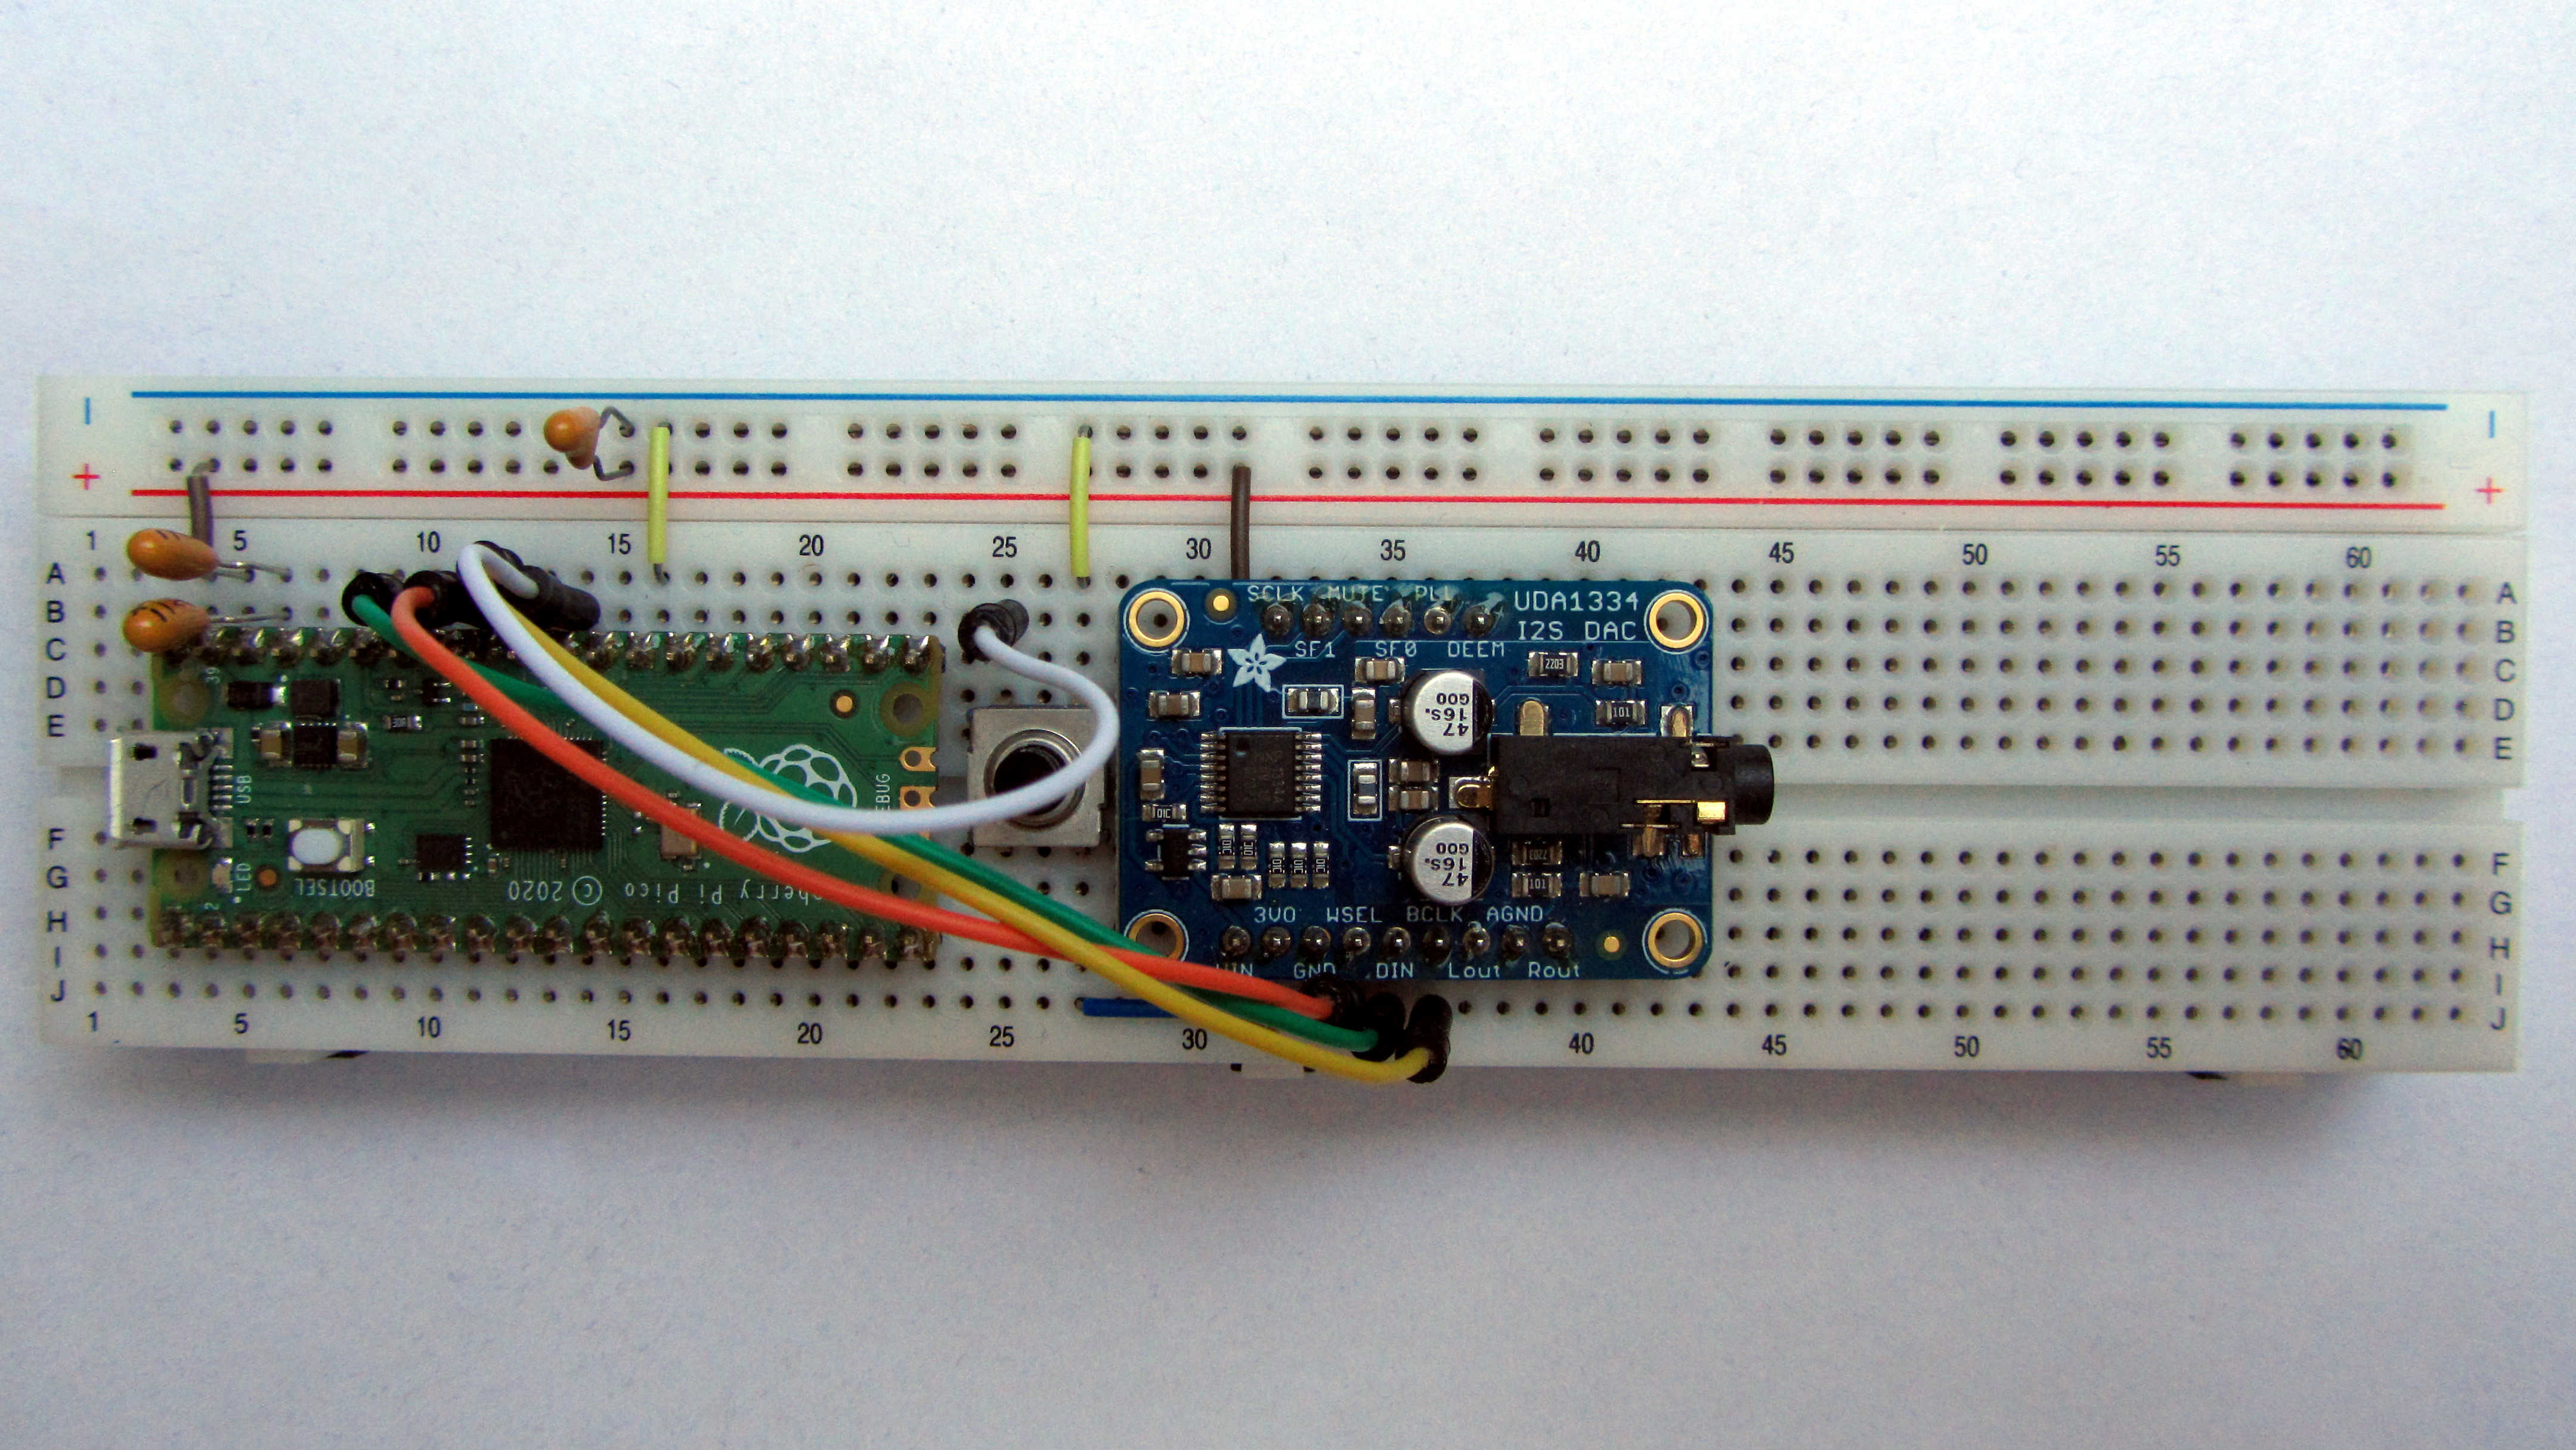
\includegraphics[width=0.75\textheight]{../../../../images/assembly-on-breadboard.jpg}<3->
  \end{center}
  \tikz[remember picture, overlay] {
    \node at (current page.south west) {
      {\color<5>{red}
        \begin{tikzpicture}[remember picture, overlay]
          \draw<5>[draw=red,thick] (4.05cm, 3.35cm) rectangle ++(0.45cm, 0.25cm);
        \end{tikzpicture}
      }
    };
    \node at (current page.south west) {
      {\color<6>{red}
        \begin{tikzpicture}[remember picture, overlay]
          \draw<6>[draw=red,thick] (5.9cm, 2.50cm) rectangle ++(1.7cm, 1.1cm);
        \end{tikzpicture}
      }
    }
  }
\end{frame}

\begin{frame}[t]{Ergebnisse \& Ausblick}
  Ergebnisse
  \begin{itemize}
  \item<2-> \color<2>{\clr} gibt sich als MIDI Device aus
  \item<3-> \color<3>{\clr} bewältigt auch vielstimmige MIDI-Ströme
  \item<4-> \color<4>{\clr} Audio-Ausgang per I²S funktioniert
  \item<5-> \color<5>{\clr} analoger Audio-Ausgang funktioniert {\em
    noch} nicht wirklich
  \item<6-> \color<6>{\clr} sehr genaue und stabile Frequenzen dank
    Bresenham
  \item<7-> \color<7>{\clr} Proof-of-Concept als Basis für komplexere
    Designs
  \item<8-> \color<8>{\clr} Quellcode (GPL-2.0):
    \url{https://github.com/soundpaint/pico-simple-stupid-synth}
  \end{itemize}
  Ausblick
  \begin{itemize}
  \item<9-> \color<9>{\clr} getrennte Kanäle, damit Auswirkung von
    {\em Note off} auf eigenen Kanal beschränkt
  \item<10-> \color<10>{\clr} {\imply} {\em Note off}: Amplitude {\em
    korrigieren} statt pauschal auf 0 zu setzen
  \item<11-> \color<11>{\clr} Update für \texttt{usb\_descriptors.c}
    auf aktuelle Version von \texttt{tinyusb}
  \item<12-> \color<12>{\clr} vielleicht demnächst multitimbrale
    Version
  \item<13-> \color<13>{\clr} {\imply} Herausforderung: $<$ 2MB
    Flashspeicher für Soundfont
  \item<14-> \color<14>{\clr} später vielleicht deutlich komplexere
    Synthese mit Pico-Cluster
  \end{itemize}
\end{frame}

% bibliography
%\section{Literaturverweise}

\begin{frame}[t,allowframebreaks]{Literaturverweise}
  \nocite{RaspberryPiLtd24a}
  \nocite{Reuter24a}
  \nocite{Wikipedia24a}
  \nocite{MIDIAssociation24a}
  \nocite{Thach24a}
  \printbibliography
\end{frame}

%\section{Klang-Demonstration}

\begin{frame}[t]{Klang-Demonstration}
  \begin{center}
    \begin{tabular}{|l m{9cm}|}
      \hline

      MIDI-Datei & \texttt{MFO-Score-3.mid}\\\hline

      Sammlung & \texttt{magicflute-00-overture-mids.zip}\\\hline

      Quelle &
      \url{https://www.mutopiaproject.org/ftp/MozartWA/KV620/magicflute-00-overture/magicflute-00-overture-mids.zip}\\\hline

      Copyright & Public Domain\\\hline
    \end{tabular}
  \end{center}
  \vspace{2cm}
  \begin{center}
    \color{WarnColor}{\LARGE\danger}{ }{\em
      Trigger-Warnung:\\Chiptune-artiger Sound mit erhöhtem Anteil
      hoher Frequenzen (Rechteckschwingungen)}
  \end{center}
\end{frame}

\begin{frame}[t]
  \begin{center}
    \Huge{Diskussion eröffnet!}
  \end{center}
\end{frame}

% backup slides

%\section{Anhänge}

%\section*{Schaltpläne}

%\begin{frame}[fragile]{Schematics}
%  \begin{center}
%    \includegraphics[width=0.75\textheight]{../schematics/synth.eps}
%  \end{center}
%\end{frame}

\end{document}

%  Local Variables:
%    coding:utf-8
%    mode:LaTeX
%  End:
